Vistool (uvis) is a system that aims at facilitating readability and interaction with huge and complex relational datasets by allowing one to build a GUI on one hand and intuitively address and map data resources as part of this GUI on the other hand. An existing version of the system, written in C\# currently runs locally on a computer under Windows. The goal throughout this document is to demonstrate the feasibility of porting such a system in browsers and thereby making it platform agnostic. In that extent, Javascript is the de facto standard language to choose. The reference diagram in figure~\ref{img:refDiagram} clearly depicts the type of visual scenario we want to be able to produce in a browser. In addition to this we also want the solution to perform well even if the amount of graphic instances is big.

\begin{figure}
    \centering
    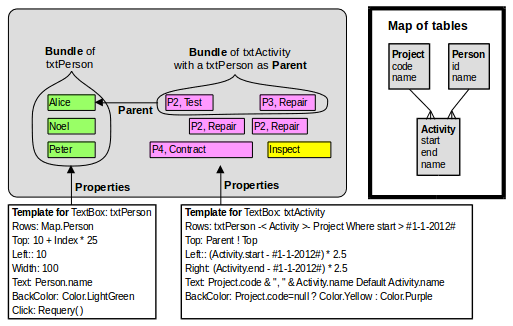
\includegraphics[width=0.9\textwidth]{images/uvisDiagram.png}
    \caption{uvis reference diagram found in the uvis card reference}
    \label{img:refDiagram}
\end{figure}

It has been decided to re-think the system as a Single Page Application, meaning that only one HTML document is loaded into the browser while the appropriate resources needed for the navigation are either provided on the document load or dynamically loaded as they are needed. Section~\ref{sec:architecture} compares the architectural differences between these architectures.

Uvis targets 3 different types of users.

\begin{itemize}
    \item The end user: a person whose interaction with the system requires no particular skill other than being able to browse to the webpage of the application
    
    \item The designer: a person with better IT knowledge. He interacts with VisTool in a privileged mode (``interaction mode'') that allow him to manipulate the set of graphical controls that are the building blocks of the application and that we refer to as the VisComponents. The designer uses the system with the end user in mind while knowing about the domain in which the system is used. 

    \item The developer is a person in charge of making the system available to the end users and the designer. He has advanced skills in IT and has the responsibility of deploying and maintaining the application. As opposed to the designer he is not required to have any knowledge about the context in which the system is used.

\end{itemize}

The whole internal logic (visEngine) is based on two initial sets of files: The vism files and the vis files.
From an users perspective, a vism file is the starting point of the application flow. As a result of loading such a file into the system he can expect to get presented with a fully operable GUI. The vism file contains information that can be described in 3 categories:

\begin{enumerate}
    \item A header that provides general information to the system. Amongst others, what visfile to load first;
    \item A database connection string;
    \item A description of the database schema
\end{enumerate}

The vis files contains the actual template-code describing how the GUI should look like.

The building process of the GUI can be roughly divided into 2 parts:
\begin{itemize}
    \item A preparation phase where a set of in-memory maps are dynamically constructed based on the text strings provided in the vism and vis files.
    \item An evaluation phase where the actual expressions mentioned in the files can be evaluated upon the content in the dynamically generated maps.
\end{itemize}

In the existing version of the application (running locally on a computer), a vism file is loaded by the visEngine through the operating system's file dialog that gives access to all files in the current user space on that particular file system. In our case where the application should be executed in the browser, the question of how and where to download the files arises. This question is tightly related to the system's architecture and is discussed in the next chapter.